\newcounter{Rcounter}
\newcommand{\sorSzamR}{\stepcounter{Rcounter}\theRcounter}

\section{Regisztráció}


A regisztráció során biztosítanunk kell szerepköröket ${Sz}_{sz\acute{a}m}$, amivel kategorizálni tudjuk a felhasználókat (\kovAzon{R\_\sorSzamR}). A felhasználóknak két csoportját különböztetjük meg: szakemberek és ügyfelek. Egy felhasználó egyszerre mindkét csoportba is tartozhat, ekkor külön nézet választóra lesz szükség (\kovAzon{R\_\sorSzamR}). További szerepkör az adminisztrátor (oldal üzemeltetés), ezen szerepkörbe tartozó személyeknek validálniuk kell a kivitelező által beállított kompetenciák, korábbi referenciák hitelességét (\kovAzon{R\_\sorSzamR}).

\subsection{Szerepkörök}

\begin{itemize}
    \item ${Sz}_1$: Szakember
    \item ${Sz}_2$: Ügyfél
    \item ${Sz}_3$: Adminisztrátor
\end{itemize}

A szükséges adatok ${SA}_{sz\acute{a}m}$ közül minden felhasználónak kötelező a név, életkor és email cím kitöltése (\kovAzon{R\_\sorSzamR}). Szakembereknél ezen felül megadásra kell kerülnie a kompetenciáknak, végzettségnek. Ezeket előre megadott listából tudják kiválasztani, azonban ez a lista bővíthető kell legyen adminisztrátor által. A munkatapasztalat meghatározásához is kötelező megadni bizonyos adatokat: a munkával töltött évek számát, az egyéni vagy csoportos munkák referenciáit. Ezeknek a hitelessége szintén ellenőrzésre fog kerülni az adminisztrátor által, például szerződések ellenőrzésével (\kovAzon{R\_\sorSzamR}). Szükséges még egy szerződés elfogadása és aláírása az oldal működtetőivel, amellyel biztosításra kerül a fizetési kötelezettség (\kovAzon{R\_\sorSzamR}). Opcionálisan megadható még a szakember földrajzi helyzete a könnyebb kereshetőség érdekében (\kovAzon{R\_\sorSzamR}).

\subsection{Szükséges adatok}

\begin{itemize}
    \item Minden felhasználónak:
    \begin{itemize}
        \item ${SA}_1$: Név
        \item ${SA}_2$: Életkor
        \item ${SA}_3$: Email cím
    \end{itemize}
    \item Szakembereknek ezen felül:
    \begin{itemize}
        \item ${SA}_4$: Kompetencia
        \item ${SA}_5$: Végzettség
        \item ${SA}_6$: Munkatapasztalat
        \begin{itemize}
            \item ${SA}_{6.1}$: Évek száma
            \item ${SA}_{6.2}$: Referencia
        \end{itemize}
        \item  ${SA}_7$: Profilkép
        \item ${SA}_8$: Földrajzi helyzet (Opcionális)
    \end{itemize}
\end{itemize}

A regisztráció során egyedi felhasználó nevet, illetve egy megfelelő erősségű jelszót kell megadnia az új felhasználónak, ami alapján egyértelműen azonosítani lehet, illetve biztonságosan be tud lépni a fiókjába (\kovAzon{R\_\sorSzamR}).

\subsection{Jelszó kritériumai}

\begin{itemize}
    \item $J_1$: legalább 8 karakter hosszúságú
    \item $J_2$: legalább 1 szám értéket tartalmaz
    \item $J_3$: legalább 1 speciális karaktert tartalmaz
    \item $J_4$: legalább 1 nagy és 1 kisbetűt tartalmaz
    \item $J_5$: kétszer meg kell adni ugyanazt a jelszót
\end{itemize}

\subsection{Felhasználónév kritériumai}

\begin{itemize}
    \item $F_1$: egyedinek kell lennie
    \item $F_2$: nem szerepelhet benne sértő szó
\end{itemize}

A regisztráció során szükség van az általános szerződési feltételek elfogadására (\kovAzon{R\_\sorSzamR}).

\subsection{ÁSZF}

\begin{itemize}
    \item $A_1$: Az ÁSZF-nek elérhetőnek kell lennie (\kovAzon{R\_\sorSzamR}).
    \item $A_2$: A felhasználónak ki kell pipálnia egy jelölőnégyzetet, amivel kijelenti, hogy megismerte és elfogadta a szerződésben foglaltakat (\kovAzon{R\_\sorSzamR}).
\end{itemize}

A regisztráció végén a felhasználó kap egy email értesítést, amivel meg kell erősítenie a regisztráció során megadott email címet (\kovAzon{R\_\sorSzamR}).

\begin{figure}[h]
	\centering
	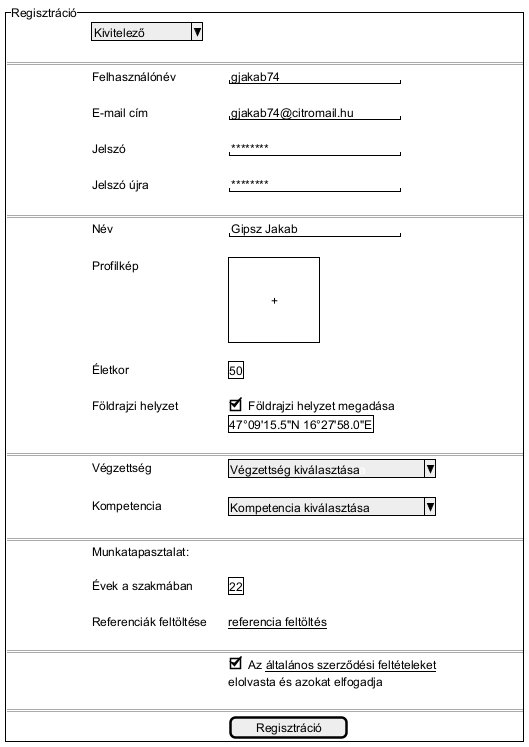
\includegraphics[scale=0.5]{img/regisztracio.png}
	\caption{Regisztráció}
	\label{fig:reg}
\end{figure}